% Generated on 2023-04-17 10:14:53 by gEcon ver. 1.2.1 (2023-01-18)
% http://gecon.r-forge.r-project.org/

% Model name: RSWTV

\section{Steady-state values}


\begin{tabular}{c|c|}
  & Steady-state value\\
\hline
${i\!H}$ & 1 \\
${i\!L}$ & 1 \\
$\lambda^{\mathrm{HIGHREGIME}^{\mathrm{1}}}$ & 0 \\
$\lambda^{\mathrm{LOWREGIME}^{\mathrm{1}}}$ & 0 \\
$\lambda^{\mathrm{HIGHREGIME}^{\mathrm{2}}}$ & 0 \\
$\lambda^{\mathrm{LOWREGIME}^{\mathrm{2}}}$ & 0 \\
${p\!i\!H}$ & 0 \\
${p\!i\!L}$ & 0 \\
${r\!n}$ & 1 \\
${y\!H}$ & 0 \\
${y\!L}$ & 0 \\
${U\!H}$ & 0 \\
${U\!L}$ & 0 \\
\hline
\end{tabular}


\section{The solution of the 1st order perturbation}

\subsection*{Matrix $P$}

$$\bordermatrix{
~ & {i\!H}_{t-1} & {i\!L}_{t-1} & {p\!i\!H}_{t-1} & {p\!i\!L}_{t-1} & {r\!n}_{t-1} & {y\!H}_{t-1} & {y\!L}_{t-1} \cr
{i\!H}_{t} & -3.2558 & 1.3136 & 10.1087 & -4.2866 & 2.8922 & -5.7473 & 2.3702 \cr
{i\!L}_{t} & 1.3136 & -3.2558 & -4.2866 & 10.1087 & 2.8922 & 2.3702 & -5.7473 \cr
{p\!i\!H}_{t} & 0 & 0 & 1.6074 & -0.5973 & 0 & -0.3962 & 0.1472 \cr
{p\!i\!L}_{t} & 0 & 0 & -0.5973 & 1.6074 & 0 & 0.1472 & -0.3962 \cr
{r\!n}_{t} & 0 & 0 & 0 & 0 & 0.95 & 0 & 0 \cr
{y\!H}_{t} & 1.5914 & -0.5913 & -1.6074 & 0.5973 & -1.0001 & 1.9875 & -0.7385 \cr
{y\!L}_{t} & -0.5913 & 1.5914 & 0.5973 & -1.6074 & -1.0001 & -0.7385 & 1.9875 \cr
}$$

\subsection*{Matrix $Q$}

$$\bordermatrix{
~ & \epsilon^{\mathrm{Z}} \cr
{i\!H} & 1 \cr
{i\!L} & 1 \cr
{p\!i\!H} & 0 \cr
{p\!i\!L} & 0 \cr
{r\!n} & 1 \cr
{y\!H} & 0 \cr
{y\!L} & 0 \cr
}$$

\subsection*{Matrix $R$}

$$\bordermatrix{
~ & {i\!H}_{t-1} & {i\!L}_{t-1} & {p\!i\!H}_{t-1} & {p\!i\!L}_{t-1} & {r\!n}_{t-1} & {y\!H}_{t-1} & {y\!L}_{t-1} \cr
\lambda^{\mathrm{HIGHREGIME}^{\mathrm{1}}}_{t} & -2.0087 & 1.3222 & 12.1149 & -7.4425 & 0.6865 & -4.9948 & 3.1567 \cr
\lambda^{\mathrm{LOWREGIME}^{\mathrm{1}}}_{t} & 1.3222 & -2.0087 & -7.4425 & 12.1149 & 0.6865 & 3.1567 & -4.9948 \cr
\lambda^{\mathrm{HIGHREGIME}^{\mathrm{2}}}_{t} & 0.4652 & -0.2856 & -2.0085 & 1.3221 & -0.1796 & 0.9602 & -0.6115 \cr
\lambda^{\mathrm{LOWREGIME}^{\mathrm{2}}}_{t} & -0.2856 & 0.4652 & 1.3221 & -2.0085 & -0.1796 & -0.6115 & 0.9602 \cr
{U\!H}_{t} & 0 & 0 & 0 & 0 & 0 & 0 & 0 \cr
{U\!L}_{t} & 0 & 0 & 0 & 0 & 0 & 0 & 0 \cr
}$$

\subsection*{Matrix $S$}

$$\bordermatrix{
~ & \epsilon^{\mathrm{Z}} \cr
\lambda^{\mathrm{HIGHREGIME}^{\mathrm{1}}} & 0 \cr
\lambda^{\mathrm{LOWREGIME}^{\mathrm{1}}} & 0 \cr
\lambda^{\mathrm{HIGHREGIME}^{\mathrm{2}}} & 0 \cr
\lambda^{\mathrm{LOWREGIME}^{\mathrm{2}}} & 0 \cr
{U\!H} & 0 \cr
{U\!L} & 0 \cr
}$$


\section{Model statistics}

\subsection{Basic statistics}

\begin{tabular}{c|c|c|c|c|}
  & Steady-state value & Std. dev. & Variance & Loglin\\
\hline
${i\!H}$ & 1.0001 & 0.1303 & 0.017 & Y    \\
${i\!L}$ & 1.0001 & 0.1303 & 0.017 & Y    \\
$\lambda^{\mathrm{HIGHREGIME}^{\mathrm{1}}}$ & 0 & 0 & 0 & N    \\
$\lambda^{\mathrm{LOWREGIME}^{\mathrm{1}}}$ & 0 & 0 & 0 & N    \\
$\lambda^{\mathrm{HIGHREGIME}^{\mathrm{2}}}$ & 0 & 0 & 0 & N    \\
$\lambda^{\mathrm{LOWREGIME}^{\mathrm{2}}}$ & 0 & 0 & 0 & N    \\
${p\!i\!H}$ & 0 & 0 & 0 & N    \\
${p\!i\!L}$ & 0 & 0 & 0 & N    \\
${r\!n}$ & 1.0001 & 0.1303 & 0.017 & Y    \\
${y\!H}$ & 0 & 0 & 0 & N    \\
${y\!L}$ & 0 & 0 & 0 & N    \\
${U\!H}$ & 0 & 0 & 0 & N    \\
${U\!L}$ & 0 & 0 & 0 & N    \\
\hline
\end{tabular}


\subsection{Correlation matrix}

\begin{tabular}{c|ccc|}
  & ${i\!H}$ & ${i\!L}$ & ${r\!n}$\\
\hline
${i\!H}$ & 1 & 1 & 1 \\
${i\!L}$ &  & 1 & 1 \\
${r\!n}$ &  &  & 1 \\
\hline
\end{tabular}


\subsection{Cross correlations with the reference variable (${i\!H}$)}

\begin{tabular}{c|c|c|c|c|c|c|c|c|c|c|c|c|}
  & $\sigma[\cdot]$ rel. to $\sigma[{i\!H}]$ & ${i\!H}_{t-5}$ & ${i\!H}_{t-4}$ & ${i\!H}_{t-3}$ & ${i\!H}_{t-2}$ & ${i\!H}_{t-1}$ & ${i\!H}_{t}$ & ${i\!H}_{t+1}$ & ${i\!H}_{t+2}$ & ${i\!H}_{t+3}$ & ${i\!H}_{t+4}$ & ${i\!H}_{t+5}$\\
\hline
${i\!H}_{t}$ & 1 & -0.016 & 0.11 & 0.271 & 0.471 & 0.713 & 1 & 0.713 & 0.471 & 0.271 & 0.11 & -0.016 \\
${i\!L}_{t}$ & 1 & -0.016 & 0.11 & 0.271 & 0.471 & 0.713 & 1 & 0.713 & 0.471 & 0.271 & 0.11 & -0.016 \\
${r\!n}_{t}$ & 1 & -0.016 & 0.11 & 0.271 & 0.471 & 0.713 & 1 & 0.713 & 0.471 & 0.271 & 0.11 & -0.016 \\
\hline
\end{tabular}


\subsection{Autocorrelations}

\begin{tabular}{c|ccccc|}
  & Lag 1 & Lag 2 & Lag 3 & Lag 4 & Lag 5\\
\hline
${i\!H}$ & 0.713 & 0.471 & 0.271 & 0.11 & -0.016 \\
${i\!L}$ & 0.713 & 0.471 & 0.271 & 0.11 & -0.016 \\
${r\!n}$ & 0.713 & 0.471 & 0.271 & 0.11 & -0.016 \\
\hline
\end{tabular}



\pagebreak

\section{Impulse response functions}

\begin{figure}[h]
\begin{minipage}{0.5\textwidth}
\vspace*{-3em}
\centering
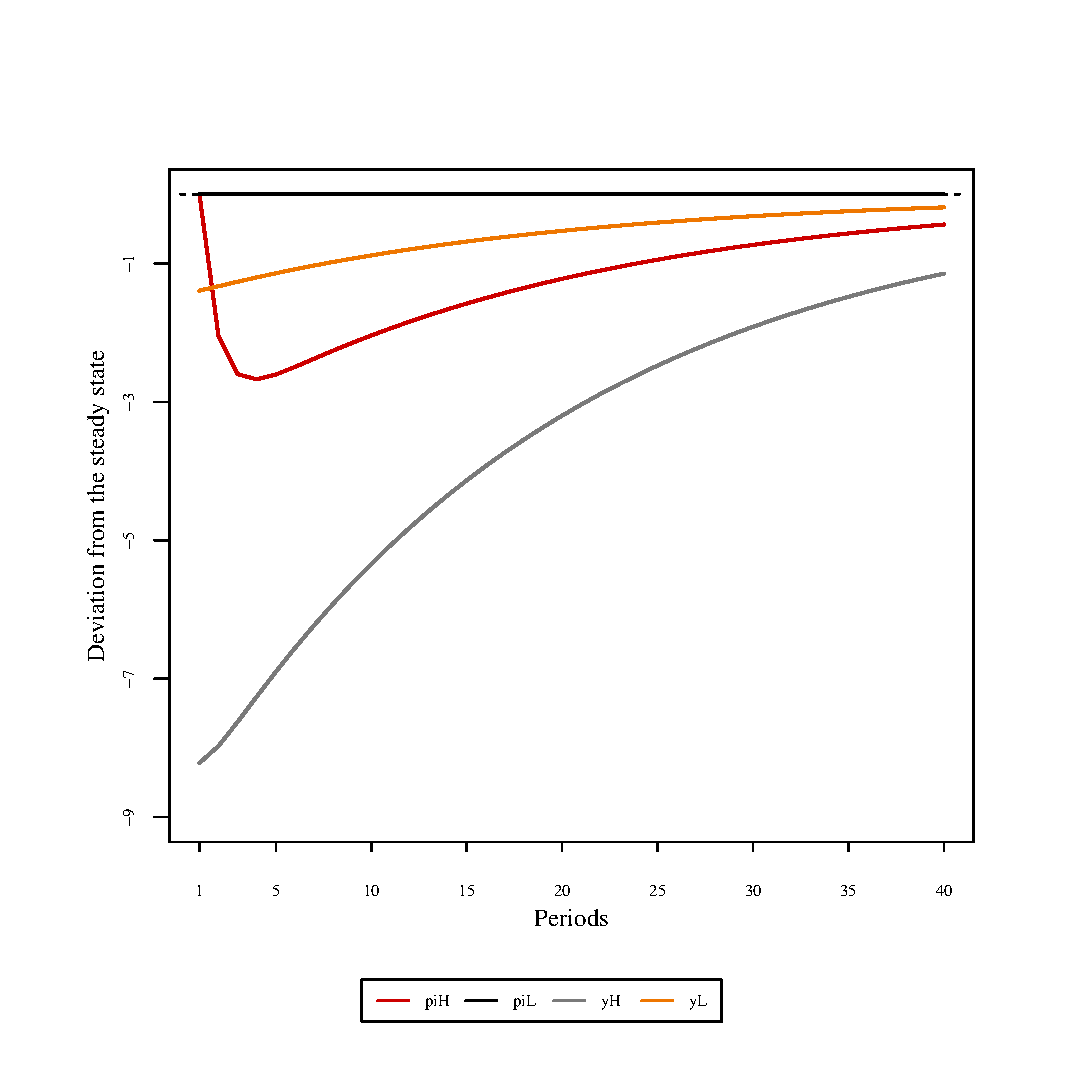
\includegraphics[width=0.99\textwidth, scale=0.55]{plots/plot_7.eps}
\caption{Impulse responses (${i\!H}, {i\!L}, {p\!i\!H}, {p\!i\!L}, {y\!H}$) to $\epsilon^{\mathrm{Z}}$ shock}
\end{minipage}
\begin{minipage}{0.5\textwidth}
\vspace*{-3em}
\centering
\includegraphics[width=0.99\textwidth, scale=0.55]{plots/plot_8.eps}
\caption{Impulse response (${y\!L}$) to $\epsilon^{\mathrm{Z}}$ shock}
\end{minipage}
\end{figure}


